\chapter{Gráficos do Experimento 3}
\subsubsection{Algoritmo Genético Geracional Clásico}

\begin{figure}[H]
\centering

\includegraphics[scale=1]{apxC/agcc/1}

\end{figure}

\begin{figure}[H]
\centering

\includegraphics[scale=1]{apxC/agcc/2}

\end{figure}

\begin{figure}[H]
\centering

\includegraphics[scale=1]{apxC/agcc/3}

\end{figure}

\begin{figure}[H]
\centering

\includegraphics[scale=1]{apxC/agcc/4}

\end{figure}

\begin{figure}[H]
\centering

\includegraphics[scale=1]{apxC/agcc/5}

\end{figure}

\begin{figure}[H]
\centering

\includegraphics[scale=1]{apxC/agcc/6}

\end{figure}

\begin{figure}[H]
\centering

\includegraphics[scale=1]{apxC/agcc/7}

\end{figure}

\begin{figure}[H]
\centering

\includegraphics[scale=1]{apxC/agcc/8}

\end{figure}

\begin{figure}[H]
\centering

\includegraphics[scale=1]{apxC/agcc/9}

\end{figure}

\begin{figure}[H]
\centering

\includegraphics[scale=1]{apxC/agcc/10}

\end{figure}

Algoritmo Genético de Regime Permanente

\begin{figure}[H]
\centering

\includegraphics[scale=1]{apxC/agrpc/1}

\end{figure}

\begin{figure}[H]
\centering

\includegraphics[scale=1]{apxC/agrpc/2}

\end{figure}
\begin{figure}[H]
\centering

\includegraphics[scale=1]{apxC/agrpc/3}

\end{figure}
\begin{figure}[H]
\centering

\includegraphics[scale=1]{apxC/agrpc/4}

\end{figure}
\begin{figure}[H]
\centering

\includegraphics[scale=1]{apxC/agrpc/5}

\end{figure}
\begin{figure}[H]
\centering

\includegraphics[scale=1]{apxC/agrpc/6}

\end{figure}
\begin{figure}[H]
\centering

\includegraphics[scale=1]{apxC/agrpc/7}

\end{figure}
\begin{figure}[H]
\centering

\includegraphics[scale=1]{apxC/agrpc/8}

\end{figure}
\begin{figure}[H]
\centering

\includegraphics[scale=1]{apxC/agrpc/9}

\end{figure}
\begin{figure}[H]
\centering

\includegraphics[scale=1]{apxC/agrpc/10}

\end{figure}